\documentclass{article}
\usepackage{amsmath}
\usepackage{caption}
\usepackage{placeins}
\usepackage{graphicx}
\usepackage{subcaption}
\usepackage{tikz}
%\usepackage[active,tightpage]{preview}
\usepackage{natbib}
\bibpunct{(}{)}{,}{a}{}{;} 
\usepackage{url}
\usepackage{nth}
\usepackage{authblk}
% for the d in integrals
\newcommand{\dd}{\; \mathrm{d}}
\newcommand{\tc}{\quad\quad\text{,}}
\newcommand{\tp}{\quad\quad\text{.}}
\defcitealias{HMD}{HMD}

\begin{document}

\title{Distributional aspects of time to death in human populations}

\author[1]{Tim Riffe\thanks{triffe@demog.berkeley.edu}}
\author[2,3]{Adam Lenart}
\author[2,3]{Vladimir Canudas Romo}
\affil[1]{Department of Demography, University of California, Berkeley}
\affil[2]{University of Southern Denmark}
\affil[3]{Max Planck Odense Center}


\maketitle

\begin{abstract}
All lifetable summary measures can be reworked as functions of conditional
remaining lifetime to become functions of age. In this paper, we provide
some elementary definitions of functions describing the conditional lifespan
distribution, and apply these to human populations.
We suggest a selection of applications and some heuristics for late life
decisions based on these distributional measures.
\end{abstract}


\section*{Background}

Typically demographers are satisfied to summarize the remaining lifetime for age
groups using a mean, $e(a)$, which is however not an omnibus descriptor of time
to death. There are other useful measures of longevity, such as
the modal or median ages at death, and demographers also have a battery of
indicators for lifespan variability or entropy. One aspect in common for many
such indicators is that they refer to the age distribution of mortality in a snapshot of a stationary population or else the age at death distribution of a newborn cohort under constant mortality
conditions. These measures are not typically made conditional on survival to
later ages, i.e., demographers too seldom consider the properties of the
distribution of remaining lifetimes as a function of age itself. 

It is our impression that mortality transitions have most
often been described in terms of changes in the mortality hazard curve, except
when framed in terms of compression \citep[e.g.,][]{fries1980aging}, which is a
distributional observation.
Hazards are attractive because rates in a given
age group can be imagined as independent from other ages. Research on
the deaths distribution (or else its translation as a survival curve) has either
been based on the entire age range
\citep[e.g.,][]{wilmoth1999rectangularization, engelman2010implications}
or else on left-censored distributions, in order to focus on senescent processes.  For instance, \citet{edwards2005inequality}
and \citet{gillespie2014divergence} left-censor analyses at
ages 10 and 15, respectively, in order to observe the deaths distribution
without a preponderance of infant mortality. Another family of studies
left-censors at variable ages, depending on the age-specific value of some
function. For example, \citet{romo2009maximum} document historical trends in
total maximum lifespan expectancy using in each instance the age that maximizes 
conditional lifespan expectancy, $a + e(a)$ (this was not
always $e(0)$). Left-censoring is also common practice in studies of old-age
mortality.
\citet{kannisto2001mode} suggested measuring old-age mortality dispersion by
left-censoring at the modal age of death, and several researchers have followed
suit \citep[e.g.,][among others]{Thatcher_22_17,Ouellette_25_19}. One could in
practice repeat such analyses after left-censoring on each age in succession, thereby
revealing an age pattern to the subject of interest (variation, inequality, and
between-population divergence) in order to form a more complete picture over
the lifecourse.

All lifetable
summary measures can be reworked as functions of conditional remaining lifetime
(e.g., the modal remaining lifespan) to become functions of age.
In this paper, we provide some elementary definitions of age-conditioned
distribution functions, including variance, skewness and kurtosis, and we apply
these to human populations from the Human Mortality Database \citepalias{HMD}.
As an example of the utility of this perspective we suggest a selection of
simple heuristics for late life decisions based on these distributional measures.

\section*{Definitions}

Remaining life expectancy conditional on survial to age $a$ is defined as
\begin{equation}
e(a) = \frac{\int_0^\infty l(a+y) \dd y}{l(a)} \tp
\end{equation}

Say lifespans for a given birth cohort are measured with the random variable,
$X$, with distribution $d(X)$, which is identical to the $d_x$
column of the lifetable if a radix of 1 is used. In other words, the
distribution of lifespans for newborns is identical to the distribution of
age at death in the stationary population. We are interested in the
conditional density function, $f(X-a ~|~ X \ge a)$, which we denote using
$f(y|a)$, where $a$ is age attained and $y$ is remaining years of life, and
which is defined as:
\begin{equation}
\label{eq:fya}
f(y|a) = \mu(a+y) \frac{l(a+y)}{l(a)} \tc
\end{equation}
i.e., the probability of surviving to and dying at age $a+y$ given survival to
age $a$. \eqref{eq:fya} can also be used to calculate remaining life expectancy:
\begin{equation}
e(a) = \int _{y=0}^\infty y f(y|a) \dd y \tp
\end{equation}

Demographers make less frequent
reference to $f(y|a)$, which is however useful for decomposing
demographic counts into remaining lifetime classes. The conditional distribution of remaining lifetimes can be
described empirically using quantiles, or other central measures such as the
median or the mode, or perhaps more parsimoniously using standardized moments.

The $n^{th}$ standardized moment about the conditional mean of $f(y|a)$,
$\eta_n(y|a)$ is defined as:
\begin{align}
\eta _n(y|a) =& \frac{1}{l(a)} \int_{y=0}^\infty (y-e(a))^n \mu (a+y) l(a+y) \dd
y 
\intertext{or just}
\eta _n(y|a) =&  \int_{y=0}^\infty (y-e(a))^n f(y|a) \dd y \tc
\end{align}
where $\eta_2(y|a)$ gives the variance of remaining lifespan about $e(a)$,
$\sigma^2(y|a)$. Survival-conditioned variance is useful
information, but it can be deceptive to display graphically, since lifespan variation is not usually symmetric around $e(a)$. The conditional skewness function, $Skew(y|a)$ is not a perfect measure of symmetry in $f(y|a)$, but it
captures most such variation and can be roughly interpreted in this way. It is
defined as
\begin{equation}
\label{eq:skew}
Skew(y|a) = \frac{\eta _3(y|a)}{\sigma(y|a)^3} \tc
\end{equation}
the third standardized moment. The conditional
kurtosis of $f(y|a)$, $Kurt(y|a)$, can be defined as
\begin{equation}
\label{eq:kurt}
Kurt(y|a) = \frac{\eta_4(y|a)}{\sigma(y|a)^4}-3 \tp
\end{equation}
The age pattern of kurtosis describes how the peakedness, or the fatness of the
tails of the remaining distribution change over age. The coefficient of
variation of remaining lifespan, $CV(y|a)$ is then simply
\begin{equation}
CV(y|a) = \frac{\sigma(y|a)}{e(a)} \tp
\end{equation}
$CV(y|a)$ is dimensionless and comparable over age, and its reciprocal
can be thought of as a signal to noise ratio of one's likely remaining lifespan,
assuming a constant mortality pattern in ages higher than $a$.

%L-moments\citep{hosking1990moments} may also be calculated for the the
% lifetable conditional distribution of remaining lifetimes. These measures yield qualitatively similar reslts, but
%are more robust to noise and outliers, and they are also appropriate for
% ordered vaiables such as age-classified mortality functions. Tyically L-moment
%calculation proceeds from individual-level data, which is never drawn from
%a stationary population. Here we present the general L-moment formulas for
%grouped data, which can be applied to the standard lifetable if specified with
% a large radix, such as the HMD standard of $100,000$, or possibly more
%appropriately to a radix the size of the theoretical stationay birth cohort
%that would yield the same popuation size as that observed in the year to which
%the lifetable refers (Adam, am I way off?).

%definition goes here:

\section*{Observed patterns}
The above definitions are exact and amenable to calculation from
the standard lifetable. We illustrate using the long series of Swedish data
available from the HMD, and provide results for other HMD populations in a
forthcoming online appendix. We begin by outlining the basic age pattern of
some interesting distribution descriptors, and continue by plotting
age-period trends as Lexis surfaces. Results show distinct transitions
according to the index viewed. The mean, standard deviation, skewness and
kurtosis occasionally suggest different onset dates. 

To
begin, let us compare some quantiles of the distribution of $f(y|a)$, translated to $f(a+y|a)$. Figure~\ref{fig:IQR} provides shows the median and interquartile range of conditional age attained implied by period rates for Swedish females in 1900 and 2000. In a general sense, we can conclude from this Figure that the lower quantiles of conditional age attained change much more over age than do upper quantiles. We also see that lower mortality regimes year (2000) have more
compact interquartile ranges than to do high mortality regimes (1900), meaning
that one can wager an age at death with greater certainty, and even earlier in
life.
Further, in contemporary low mortality regimes, with low early life mortality, the
conditional IQR holds nearly constant (in fact it always rises, albeit
imperceptibly) until after typical midlife ages.

Figure~\ref{fig:Var} is similar to Figure~\ref{fig:IQR}, but shows the mean of
conditional lifespan, $a+e(a)$, as a function of age, plus and minus a single standard deviation about $e(a)$. This might be a less useful
indicator of spread than is IQR due to assymetry, until later in life, when it
yields similar results to the IQR.
% Figure produced in R/GeneralPatterns.R

\begin{figure}[h!]
\centering
\caption{Sweden, females in 1900 \& 2000. Period mortality (HMD)}
\label{fig:IQRVar}
\begin{subfigure}[b]{.48\linewidth}
\centering
	\caption{\nth{25}, \nth{50}, and \nth{75}
	percentiles of conditional lifespan.}
	\label{fig:IQR}
	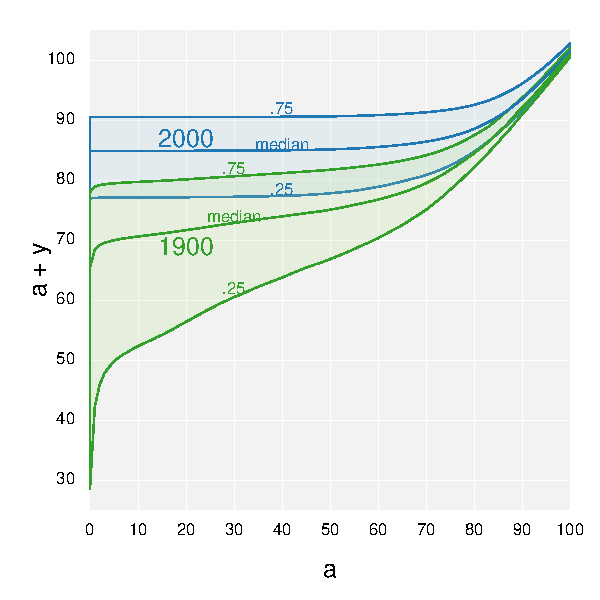
\includegraphics[scale=.65]{Figures/SwedenFemalesIQR1900_2000.pdf}	
\end{subfigure}
~
\begin{subfigure}[b]{.48\linewidth}
\centering
	\caption{Variation around mean, $e(a)+/-\sigma(y|a)$ 
	(a single standard deviation).}
	\label{fig:Var}
	\includegraphics[scale=.65]{Figures/SwedenFemalesVar1900_2000.pdf}	
\end{subfigure}
\end{figure}

\begin{figure}[h!]
\centering
\caption{Sweden, females in 1900, 1950 \& 2000. Period
	mortality (HMD).}
\label{fig:SkewKurt}
\begin{subfigure}[b]{.48\linewidth}
\caption{Skewness, $\gamma_1(y|a)$ from
	equation~\eqref{eq:skew}.}
	\label{fig:skew}
	\includegraphics[scale=.65]{Figures/SwedenFemalesSkew1900_2000.pdf}	
\end{subfigure}
~
\begin{subfigure}[b]{.48\linewidth}
\centering
	\caption{Kurtosis, $\gamma_2(y|a)$ from
	equation~\eqref{eq:kurt}.}
	\label{fig:kurt}
	\includegraphics[scale=.65]{Figures/SwedenFemalesKurt1900_2000.pdf}	
\end{subfigure}
\end{figure}

Variance can be usefully supplemented after infant mortality
has passed by referring to the skewness and kurtosis patterns over age,
displayed in Figure~\ref{fig:SkewKurt}, which also includes intermediate year,
1950. Skewness and kurtosis also display strong age patterns. Skewness,
Figure~\ref{fig:skew}, essentially increases until old-age mortality
deceleration, crossing zero somewhere the age where mean and median remaining
life expectancy are equal, and also in the neighborhood of the late-life minimum
in kurtosis, Figure~\ref{fig:kurt}. In contemporary low mortality conditions,
kurtosis follows a roller-coaster pattern over age, with positive excess
kurtosis falling from birth to become negative around age 50 or 60, then
positive again around age 80, and perhaps again negative sometime after age
100.\footnote{The observation of a platykurtic remaining lifespan distribution
after age 100 is sensitive to data quality and adjustments/ smoothing
used, and we do not analyse this in depth.} In high-mortality populations, such
as 1900 Sweden, the kurtosis of remaining lifespan remained slightly platykurtic
until between age 70 and 80.

Each distribution moment has undergone major shifts in the recorded past, which
we plot on Lexis surfaces for Swedish females for the 260 years of data
available from the HMD. Figure~\ref{fig:exLex} shows the well-known mean
remaining lifespan, $e(a)$, the isopeleths of which have maintained a steady
linear increasing pattern since at least the 1950s. Figure~\ref{fig:sdLex} shows
the standard deviation of remaining lifespan, the age pattern of which held roughly
constant for the first 150 years of data, and appears to have started an
abrupt shift, still underway, starting at the 1918 influenza pandemic.

Skewness, Figure~\ref{fig:skewLex} has undergone a much longer
transition, starting before the mid \nth{19} Century and accelerating after the 1918
pandemic. The trend has been one of decrease in all ages. Kurtosis,
Figure~\ref{fig:kurtLex}, began its transition around 1900, decreasing in ages
above $e(a)$ and increasing in ages below $e(a)$, but always obtaining a
local minimum near $e(a)$.
The coefficient of variation, Figure~\ref{fig:CVLex}, began its decreasing trend
in the \nth{19} Century, driven initially by its denominator, $e(a)$, and after 1918 by
both changes in the mean and standard deviation.

\begin{figure}
\centering
\caption{Sweden, females in 1751-2011, ages 0-110+. Period
	mortality (HMD).}
\label{fig:exsdLex}
\begin{subfigure}{1.1\textwidth}
\centering
\caption{$e(a)$, remaining life expectancy.}
\vspace{-1em}
	\label{fig:exLex}
	\makebox[\textwidth][c]{\includegraphics[scale=.6]{Figures/Surf/exSWEf.pdf}	}
\end{subfigure}
\\
\begin{subfigure}{1.1\textwidth}
\centering
	\caption{$\sigma(y|a)$, standard deviation of remaining lifespan.}
	\vspace{-1em}
	\label{fig:sdLex}
	\makebox[\textwidth][c]{\includegraphics[scale=.6]{Figures/Surf/SDSWEf.pdf}	}
\end{subfigure}
\end{figure}

\begin{figure}
\vspace{-6em}
\centering
\caption{Skewness, Kurtosis and CV of remaining lifespan.
Sweden, females in 1751-2011, ages 0-110+.
Period mortality (HMD).}
\label{fig:exsdLex}
\begin{subfigure}{1.1\textwidth}
\centering
\caption{Skewness, $Skew(y|a)$}
\vspace{-1em}
	\label{fig:skewLex}
	\makebox[\textwidth][c]{\includegraphics[scale=.6]{Figures/Surf/SskewSWEf.pdf}
	}
\end{subfigure}
\\
\begin{subfigure}{1.1\textwidth}
\centering
	\caption{Kurtosis, $Kurt(y|a)$}
	\vspace{-1em}
	\label{fig:kurtLex}
	\makebox[\textwidth][c]{\includegraphics[scale=.6]{Figures/Surf/KurtSWEf.pdf}	}
\end{subfigure}
\\
\begin{subfigure}{1.1\textwidth}
\centering
	\caption{Coefficient of Variation, $CV(y|a)$}
	\vspace{-1em}
	\label{fig:CVLex}
	\makebox[\textwidth][c]{\includegraphics[scale=.6]{Figures/Surf/CVSWEf.pdf}	}
\end{subfigure}
\end{figure}
\FloatBarrier

Data and code used to produce these results will be made available, and an
appendix of results for other HMD populations and both sexes will also be made
available.

\section*{Heuristics}
(section in progress)

Distributional aspects of age-conditioned mortality may play a decisive role
in designing lifespan-related policies, interventions, hedges, and investments.
By lifespan-related, we refer both to policies that affect and are affected by
lifespan. For instance, \citet{edwards2013cost} derives an abstract approach to
estimate or conceive of a cost to variance in human lifespan. This work was
based on the lifetable deaths distribution as a whole, but we pose the question
that perhaps a) there are costs and opportunities implicit in other moments and
b) these costs may vary depending on the age of the beholder, and may not be implicit and
homogenous over all ages. Choices, such as the decision to
preemptively move into a care residence, are age dependant, and the age pattern
of optimal behavior may hinge on mortality projected in ages higher than $a$.

The empirical distribution
of $f(y|a)$ bears heavily on the consequences of many late-life
decisions (in the aggregate), and so should help shape individual planning.
Application domains include purchaser evaluations of life insurace, the decision to bequest, or the decision to pre-emptively move into a care
residence. While the sustainability of pension and retirement plans is
mostly a function of mean remaining lifetime, their equality with respect to
post-labor lifespan depends on $f(y|a)$ for the general population and for
subpopulations. To equalize the duration of retirement between
individuals is at first glance a step toward equality, but there is no necessary or best
way to determine this duration, and there is also no necessary way to adjust
this duration as a function of lifespan itself. In other words, if the desired
duration of retirement is 20 years, perhaps the meaning of 20 years is greater for an individual with a shorter lifespan and lesser for a longer total lifespan. Whether the goal is to equalize the duration of retirement, the proportion of life in retirement, or some other way of partitioning lifelines into lifecourse stages, distributional aspects of lifespans hold promise as an element in formulating analytic guidelines. Distributional differences between population subgroups vary greatly, as we demonstrate for sex differences. Sex differences and differences between other population subgroups may form the basis for research on group differences in
the lifespan distribution. 


\bibliographystyle{plainnat}
  \bibliography{references}   % Use the BibTeX file ``References.bib''.

\end{document}
